\documentclass[11pt,a4paper]{report}
\usepackage[textwidth=37em,vmargin=30mm]{geometry}
\usepackage{calc,xunicode,amsmath,amssymb,paralist,enumitem,tabu,booktabs,datetime2,xeCJK,xeCJKfntef,listings}
\usepackage{tocloft,fancyhdr,tcolorbox,xcolor,graphicx,eso-pic,xltxtra,xelatexemoji}

\newcommand{\envyear}[0]{2025}
\newcommand{\envdatestr}[0]{2025-02-13}
\newcommand{\envfinaldir}[0]{webdb/2025/20250213/final}

\usepackage[hidelinks]{hyperref}
\hypersetup{
    colorlinks=false,
    pdfpagemode=FullScreen,
    pdftitle={Web Digest - \envdatestr}
}

\setlength{\cftbeforechapskip}{10pt}
\renewcommand{\cftchapfont}{\rmfamily\bfseries\large\raggedright}
\setlength{\cftbeforesecskip}{2pt}
\renewcommand{\cftsecfont}{\sffamily\small\raggedright}

\setdefaultleftmargin{2em}{2em}{1em}{1em}{1em}{1em}

\usepackage{xeCJK,xeCJKfntef}
\xeCJKsetup{PunctStyle=plain,RubberPunctSkip=false,CJKglue=\strut\hskip 0pt plus 0.1em minus 0.05em,CJKecglue=\strut\hskip 0.22em plus 0.2em}
\XeTeXlinebreaklocale "zh"
\XeTeXlinebreakskip = 0pt


\setmainfont{Brygada 1918}
\setromanfont{Brygada 1918}
\setsansfont{IBM Plex Sans}
\setmonofont{JetBrains Mono NL}
\setCJKmainfont{Noto Serif CJK SC}
\setCJKromanfont{Noto Serif CJK SC}
\setCJKsansfont{Noto Sans CJK SC}
\setCJKmonofont{Noto Sans CJK SC}

\setlength{\parindent}{0pt}
\setlength{\parskip}{8pt}
\linespread{1.15}

\lstset{
	basicstyle=\ttfamily\footnotesize,
	numbersep=5pt,
	backgroundcolor=\color{black!5},
	showspaces=false,
	showstringspaces=false,
	showtabs=false,
	tabsize=2,
	captionpos=b,
	breaklines=true,
	breakatwhitespace=true,
	breakautoindent=true,
	linewidth=\textwidth
}






\newcommand{\coverpic}[2]{
    % argv: itemurl, authorname
    Cover photo by #2~~(\href{#1}{#1})
}
\newcommand{\makeheader}[0]{
    \begin{titlepage}
        % \newgeometry{hmargin=15mm,tmargin=21mm,bmargin=12mm}
        \begin{center}
            
            \rmfamily\scshape
            \fontspec{BaskervilleF}
            \fontspec{Old Standard}
            \fontsize{59pt}{70pt}\selectfont
            WEB\hfill DIGEST
            
            \vfill
            % \vskip 30pt
            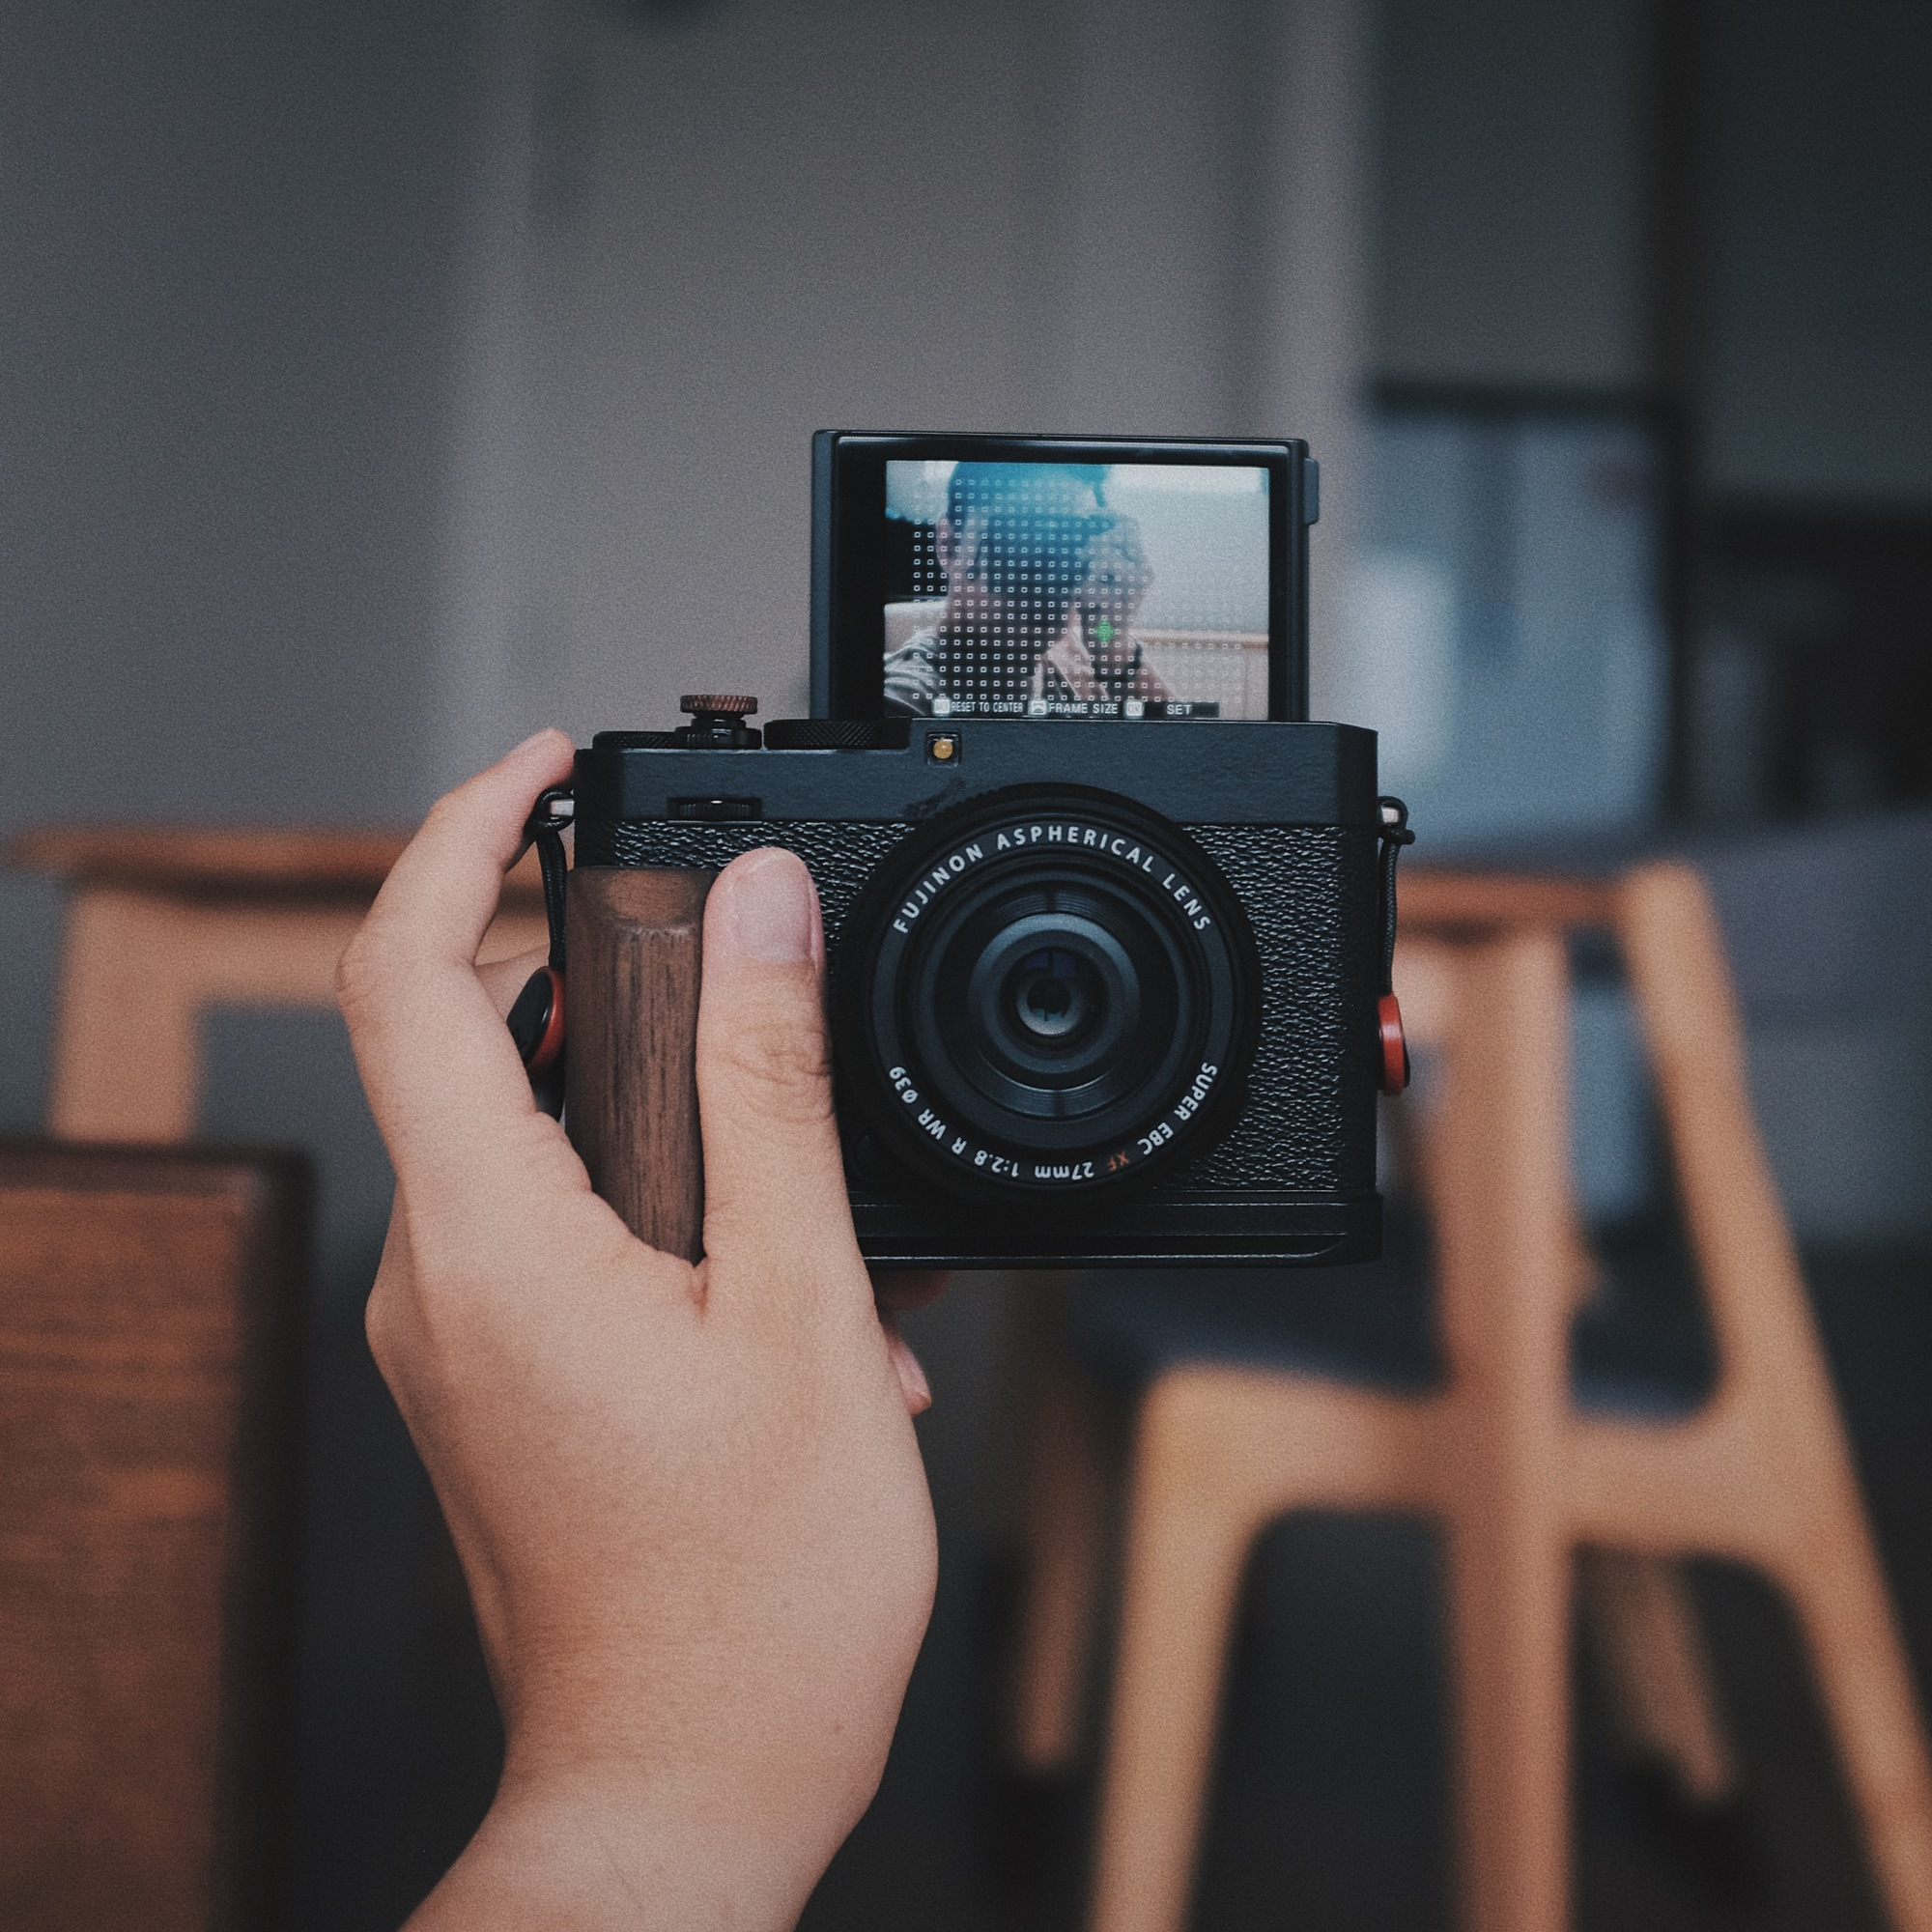
\includegraphics[width=\linewidth]{\envfinaldir/coverpic-prod.jpg}\par
            % \vskip 30pt
            \vfill

            \normalsize\rmfamily\scshape
            \copyright{} The Web Digest Project \hfill\large \envdatestr
        \end{center}
    \end{titlepage}
    % \restoregeometry
}
\newcommand{\simplehref}[1]{%
    \textcolor{blue!80!green}{\href{#1}{#1}}%
}
\renewcommand{\contentsname}{\center\Huge\sffamily\bfseries Contents\par\vskip 20pt}
\newcounter{ipartcounter}
\setcounter{ipartcounter}{0}
\newcommand{\ipart}[1]{
    % \vskip 20pt
    \clearpage
    \stepcounter{ipartcounter}
    \phantomsection
    \addcontentsline{toc}{chapter}{#1}
    % \begin{center}
    %     \Huge
    %     \sffamily\bfseries
    %     #1
    % \end{center}
    % \vskip 20pt plus 7pt
}
\newcounter{ichaptercounter}
\setcounter{ichaptercounter}{0}
\newcommand{\ichapter}[1]{
    % \vskip 20pt
    \clearpage
    \stepcounter{ichaptercounter}
    \phantomsection
    \addcontentsline{toc}{section}{\numberline{\arabic{ichaptercounter}}#1}
    \begin{center}
        \Huge
        \sffamily\bfseries
        #1
    \end{center}
    \vskip 20pt plus 7pt
}
\newcommand{\entrytitlefont}[1]{\subsection*{\raggedright\Large\sffamily\bfseries#1}}
\newcommand{\entryitemGeneric}[2]{
    % argv: title, url
    \parbox{\linewidth}{
        \entrytitlefont{#1}\par\vskip 5pt
        \footnotesize\ttfamily\mdseries
        \simplehref{#2}
    }\vskip 11pt plus 11pt minus 1pt
}
\newcommand{\entryitemGithub}[3]{
    % argv: title, url, desc
    \parbox{\linewidth}{
        \entrytitlefont{#1}\par\vskip 5pt
        \footnotesize\ttfamily\mdseries
        \simplehref{#2}\par\vskip 5pt
        \small\rmfamily\mdseries#3
    }\vskip 11pt plus 11pt minus 1pt
}
\newcommand{\entryitemAp}[3]{
    % argv: title, url, desc
    \parbox{\linewidth}{
        \entrytitlefont{#1}\par\vskip 5pt
        \footnotesize\ttfamily\mdseries
        \simplehref{#2}\par\vskip 5pt
        \small\rmfamily\mdseries#3
    }\vskip 11pt plus 11pt minus 1pt
}
\newcommand{\entryitemHackernews}[3]{
    % argv: title, hnurl, rawurl
    % \parbox{\linewidth}{
    %     \entrytitlefont{#1}\par\vskip 5pt
    %     \footnotesize\ttfamily\mdseries
    %     \simplehref{#3}\par
    %     \textcolor{black!50}{\href{#2}{#2}}
    % }\vskip 11pt plus 11pt minus 1pt
    \begin{minipage}{\linewidth}
            \entrytitlefont{#1}\par\vskip 5pt
            \footnotesize\ttfamily\mdseries
            \simplehref{#3}\par
            \textcolor{black!50}{\href{#2}{#2}}
    \end{minipage}\par\vskip 11pt plus 11pt minus 1pt
}







\begin{document}

\makeheader

\tableofcontents\clearpage




\ipart{Developers}
\ichapter{Hacker News}
\entryitemTwoLinks{Show HN: Game Bub – open-source FPGA retro emulation handheld}{https://news.ycombinator.com/item?id=43027335}{https://eli.lipsitz.net/posts/introducing-gamebub/}

\entryitemTwoLinks{5G networks meet consumer needs as mobile data growth slows}{https://news.ycombinator.com/item?id=43027266}{https://spectrum.ieee.org/5g-bandwidth}

\entryitemTwoLinks{Record-breaking neutrino is most energetic ever detected}{https://news.ycombinator.com/item?id=43027150}{https://www.nature.com/articles/d41586-025-00444-1}

\entryitemTwoLinks{The Prophet of Parking: A eulogy for the great Donald Shoup}{https://news.ycombinator.com/item?id=43026920}{https://www.worksinprogress.news/p/the-prophet-of-parking}

\entryitemTwoLinks{Most-Watched Software Engineering Talks of 2024}{https://news.ycombinator.com/item?id=43026590}{https://www.techtalksweekly.io/p/100-most-watched-software-engineering}

\entryitemTwoLinks{PgAssistant: OSS tool to help devs understand and optimize PG performance}{https://news.ycombinator.com/item?id=43026036}{https://github.com/nexsol-technologies/pgassistant}

\entryitemTwoLinks{DeaDBeeF: The Ultimate Music Player}{https://news.ycombinator.com/item?id=43024961}{https://deadbeef.sourceforge.io/}

\entryitemTwoLinks{Leaking the email of any YouTube user for \$10k}{https://news.ycombinator.com/item?id=43024221}{https://brutecat.com/articles/leaking-youtube-emails}

\entryitemTwoLinks{League of Legends data scraping the hard and tedious way for fun}{https://news.ycombinator.com/item?id=43024173}{https://maknee.github.io/blog/2025/League-Data-Scraping/}

\entryitemTwoLinks{Tiny Pointers}{https://news.ycombinator.com/item?id=43023634}{https://arxiv.org/abs/2111.12800}

\entryitemTwoLinks{US and UK refuse to sign AI safety declaration at summit}{https://news.ycombinator.com/item?id=43023554}{https://arstechnica.com/ai/2025/02/us-and-uk-refuse-to-sign-ai-safety-declaration-at-summit/}

\entryitemTwoLinks{Smuggling arbitrary data through an emoji}{https://news.ycombinator.com/item?id=43023508}{https://paulbutler.org/2025/smuggling-arbitrary-data-through-an-emoji/}

\entryitemTwoLinks{Git clone –depth 2 is vastly better than –depth 1 if you want to Git push later}{https://news.ycombinator.com/item?id=43023283}{https://stackoverflow.com/questions/66431436/pushing-to-github-after-a-shallow-clone-is-horribly-slow}

\entryitemTwoLinks{A gracious end to Webb-site}{https://news.ycombinator.com/item?id=43023141}{https://webb-site.com/articles/shutdown.asp}

\entryitemTwoLinks{Tesla sales dropped 60\% in Germany}{https://news.ycombinator.com/item?id=43023110}{https://electrek.co/2025/02/05/tesla-sales-dropped-60-in-germany/}

\entryitemTwoLinks{ElevenReader}{https://news.ycombinator.com/item?id=43022398}{https://elevenreader.io}

\entryitemTwoLinks{Parents were injured in a Tesla crash. She ended up having to pay Tesla damages}{https://news.ycombinator.com/item?id=43022307}{https://apnews.com/article/tesla-china-lawsuits-musk-investigation-58b10ccace488784fcc63646ab78b410}

\entryitemTwoLinks{I wrote a static web page and accidentally started a community (2023)}{https://news.ycombinator.com/item?id=43021677}{https://localfirstweb.dev/blog/2023-05-29-i-wrote-a-static-web-page}

\entryitemTwoLinks{jj: a Git-compatible VCS that is both simple and powerful}{https://news.ycombinator.com/item?id=43021515}{https://github.com/jj-vcs/jj}

\entryitemTwoLinks{Resist Authoritarianism by Refusing to Obey in Advance (2017)}{https://news.ycombinator.com/item?id=43021333}{https://lithub.com/resist-authoritarianism-by-refusing-to-obey-in-advance/}\ichapter{Phoronix}
\entryitemGeneric{\hskip 0pt{}ARCTIC Freezer 4U-SP5 Provides Effective Cooling For AMD EPYC 9004/9005 CPUs}{https://www.phoronix.com/review/arctic-freezer-4u-sp5}

\entryitemGeneric{\hskip 0pt{}Mesa 25.0-rc3 Released With Numerous RADV \& RadeonSI Fixes}{https://www.phoronix.com/news/Mesa-25.0-rc3-Released}

\entryitemGeneric{\hskip 0pt{}Linux 6.13 Performance For 250Hz vs. 1000Hz Timer Frequency Comparison}{https://www.phoronix.com/news/Linux-250Hz-1000Hz-Kernel-2025}

\entryitemGeneric{\hskip 0pt{}GNU Shepherd 1.0.2 Service Manager Delivers Fixes}{https://www.phoronix.com/news/GNU-Shepherd-1.0.2}

\entryitemGeneric{\hskip 0pt{}Linux 6.15 To Bring More Improvements To DRM Panic "Screen of Death"}{https://www.phoronix.com/news/Linux-6.15-More-DRM-Panic}

\entryitemGeneric{\hskip 0pt{}Intel C1 Demotion Knob Proposed For The Linux Kernel To Help Newer Xeon CPUs}{https://www.phoronix.com/news/Intel-C1-Demotion-Knob-Linux}

\entryitemGeneric{\hskip 0pt{}Open-Source Qualcomm Adreno Vulkan Driver Matures To Default AArch64 Mesa Driver List}{https://www.phoronix.com/news/Mesa-25.1-Turnip-ARM64-Default}

\entryitemGeneric{\hskip 0pt{}Intel Thermal Daemon 2.5.9 Prepares For Panther Lake}{https://www.phoronix.com/news/Intel-Thermal-Daemon-2.5.9}

\entryitemGeneric{\hskip 0pt{}Python 3.14 Alpha 5 Released With New Tail-Call Interpreter}{https://www.phoronix.com/news/Python-3.14-Alpha-5}\ichapter{Dribbble}
\entryitemGeneric{\hskip 0pt{}Carbon Solutions B2B Dashboard Design}{https://dribbble.com/shots/25554521-Carbon-Solutions-B2B-Dashboard-Design}

\entryitemGeneric{\hskip 0pt{}Illustration}{https://dribbble.com/shots/25619766-Illustration}

\entryitemGeneric{\hskip 0pt{}Fintech icons pack download}{https://dribbble.com/shots/25607159-Fintech-icons-pack-download}

\entryitemGeneric{\hskip 0pt{}Self Love}{https://dribbble.com/shots/25607914-Self-Love}

\entryitemGeneric{\hskip 0pt{}Urban Echo}{https://dribbble.com/shots/25608526-Urban-Echo}

\entryitemGeneric{\hskip 0pt{}Cloaked Wireless Device}{https://dribbble.com/shots/25403560-Cloaked-Wireless-Device}

\entryitemGeneric{\hskip 0pt{}Logo tip 001. Symmetry and asymmetry}{https://dribbble.com/shots/25606111-Logo-tip-001-Symmetry-and-asymmetry}

\entryitemGeneric{\hskip 0pt{}World Peace}{https://dribbble.com/shots/25609765-World-Peace}

\entryitemGeneric{\hskip 0pt{}Sentinal - Logo Design}{https://dribbble.com/shots/25606497-Sentinal-Logo-Design}

\entryitemGeneric{\hskip 0pt{}Tanuki}{https://dribbble.com/shots/25606258-Tanuki}

\entryitemGeneric{\hskip 0pt{}Dirty Dutch - Brand Mark / Logo}{https://dribbble.com/shots/25604523-Dirty-Dutch-Brand-Mark-Logo}

\entryitemGeneric{\hskip 0pt{}Barbershop POS app for booking and payments}{https://dribbble.com/shots/25596116-Barbershop-POS-app-for-booking-and-payments}

\entryitemGeneric{\hskip 0pt{}Seam Logo Redesigned}{https://dribbble.com/shots/25595119-Seam-Logo-Redesigned}

\entryitemGeneric{\hskip 0pt{}HugNecks®}{https://dribbble.com/shots/25596356-HugNecks}

\entryitemGeneric{\hskip 0pt{}Payoneer App Concept Design}{https://dribbble.com/shots/25593820-Payoneer-App-Concept-Design}

\entryitemGeneric{\hskip 0pt{}Nimmio}{https://dribbble.com/shots/25594035-Nimmio}

\entryitemGeneric{\hskip 0pt{}Playtech Animated Icons - Payments}{https://dribbble.com/shots/25592523-Playtech-Animated-Icons-Payments}

\entryitemGeneric{\hskip 0pt{}Aphmau Cat}{https://dribbble.com/shots/25593493-Aphmau-Cat}

\entryitemGeneric{\hskip 0pt{}Cloaked Logo Design}{https://dribbble.com/shots/25585116-Cloaked-Logo-Design}

\entryitemGeneric{\hskip 0pt{}CropBytes 2d \& 3d logo}{https://dribbble.com/shots/25590388-CropBytes-2d-3d-logo}

\entryitemGeneric{\hskip 0pt{}The Journey}{https://dribbble.com/shots/25590279-The-Journey}

\entryitemGeneric{\hskip 0pt{}Easyalgos Logo Design}{https://dribbble.com/shots/25589439-Easyalgos-Logo-Design}

\entryitemGeneric{\hskip 0pt{}Tailor Brands Logo}{https://dribbble.com/shots/25590868-Tailor-Brands-Logo}

\entryitemGeneric{\hskip 0pt{}Wylder Logo Design - W letter monogram}{https://dribbble.com/shots/25589195-Wylder-Logo-Design-W-letter-monogram}


\ipart{Developers~~~~(zh-Hans)}
\ichapter{Solidot}
\entryitemGeneric{\hskip 0pt{}来自半人马座的物质可能已进入太阳系}{https://www.solidot.org/story?sid=80542}

\entryitemGeneric{\hskip 0pt{}真正的自主 AI 也许即将到来}{https://www.solidot.org/story?sid=80541}

\entryitemGeneric{\hskip 0pt{}苹果与阿里合作为国行 iPhone 提供 AI 功能 }{https://www.solidot.org/story?sid=80540}

\entryitemGeneric{\hskip 0pt{}KDE Plasma 6.3 释出}{https://www.solidot.org/story?sid=80539}

\entryitemGeneric{\hskip 0pt{}YouTube CEO 称多数用户通过电视看 YouTube}{https://www.solidot.org/story?sid=80538}

\entryitemGeneric{\hskip 0pt{}Google Chrome 将自动替换泄露的密码}{https://www.solidot.org/story?sid=80537}

\entryitemGeneric{\hskip 0pt{}Kickstarter 将就失败的项目警告用户}{https://www.solidot.org/story?sid=80536}

\entryitemGeneric{\hskip 0pt{}Tumblr 将在后端迁移到 WordPress 后加入联邦宇宙}{https://www.solidot.org/story?sid=80535}

\entryitemGeneric{\hskip 0pt{}比亚迪为低端车型配备天神之眼}{https://www.solidot.org/story?sid=80534}

\entryitemGeneric{\hskip 0pt{}CEO 称 OpenAI 不出售}{https://www.solidot.org/story?sid=80533}

\entryitemGeneric{\hskip 0pt{}苹果释出紧急更新修复 0day}{https://www.solidot.org/story?sid=80532}

\entryitemGeneric{\hskip 0pt{}DeepSeek AI 训练成本并不低}{https://www.solidot.org/story?sid=80531}

\entryitemGeneric{\hskip 0pt{}上海自研 GLP-1 糖尿病新药批准上市}{https://www.solidot.org/story?sid=80530}

\entryitemGeneric{\hskip 0pt{}微软研究发现 AI 可能会导致人类认知能力退化}{https://www.solidot.org/story?sid=80529}

\entryitemGeneric{\hskip 0pt{}美国优秀 AI 人才四成来自中国}{https://www.solidot.org/story?sid=80528}

\entryitemGeneric{\hskip 0pt{}OpenAI 预计数个月内完成自研 AI 芯片的设计}{https://www.solidot.org/story?sid=80527}

\entryitemGeneric{\hskip 0pt{}对国内大学生的研究发现锻炼有助于减轻网瘾症状}{https://www.solidot.org/story?sid=80526}

\entryitemGeneric{\hskip 0pt{}科学家发现宇宙最大结构 Quipu}{https://www.solidot.org/story?sid=80525}

\entryitemGeneric{\hskip 0pt{}感染 COVID-19 可能加速大脑衰老四年}{https://www.solidot.org/story?sid=80524}

\entryitemGeneric{\hskip 0pt{}地球内核并非完全固态}{https://www.solidot.org/story?sid=80523}\ichapter{V2EX}
\entryitemGeneric{\hskip 0pt{}[酷工作] [远程办公/全球招募/Web3 招聘] 资深后端工程师/API 支持工程师}{https://www.v2ex.com/t/1111061}

\entryitemGeneric{\hskip 0pt{}[电影] 我就想问下,论坛是不是只有我一个没有贡献哪吒票房的}{https://www.v2ex.com/t/1111060}

\entryitemGeneric{\hskip 0pt{}[生活] 碎碎念也谈相亲}{https://www.v2ex.com/t/1111058}

\entryitemGeneric{\hskip 0pt{}[问与答] 之前公司有一批项目是由外面公司开发部署维护的(每年都支付很多费用),现在想将这批项目接收回来自行管理,请问一下需要注意什么问题呢?}{https://www.v2ex.com/t/1111057}

\entryitemGeneric{\hskip 0pt{}[分享发现] 干中学独立开发访谈 02:小店会员管家 针对个体商户的会员储值记账系统}{https://www.v2ex.com/t/1111056}

\entryitemGeneric{\hskip 0pt{}[iOS] 爱思好牛啊, 有原理科普为什么可以做到, mac 系统安装个 app 到手机上,两年了,不会过期。}{https://www.v2ex.com/t/1111055}

\entryitemGeneric{\hskip 0pt{}[户外运动] 推荐一个滑雪场}{https://www.v2ex.com/t/1111054}

\entryitemGeneric{\hskip 0pt{}[分享发现] 🎉 115 网盘用户狂喜!开源神器「115Master」让你的观影体验原地起飞 🚀}{https://www.v2ex.com/t/1111053}

\entryitemGeneric{\hskip 0pt{}[分享创造] 书签管理插件 - 让你的 Chrome 书签管理更轻松}{https://www.v2ex.com/t/1111050}

\entryitemGeneric{\hskip 0pt{}[问与答] 万兴科技是不是加班巨猛?}{https://www.v2ex.com/t/1111049}

\entryitemGeneric{\hskip 0pt{}[问与答] DeepSeek 可以部署在 U 盘里面吗?}{https://www.v2ex.com/t/1111048}

\entryitemGeneric{\hskip 0pt{}[酷工作] 深圳\_SRE 工程师\_60 万\_求大厂从业经验 SRE}{https://www.v2ex.com/t/1111047}

\entryitemGeneric{\hskip 0pt{}[问与答] 互联网公司的 hr 以及行政人员搞不搞强制比例的末位淘汰?}{https://www.v2ex.com/t/1111046}

\entryitemGeneric{\hskip 0pt{}[程序员] web 3.0 要来了,那什么是 web 3.0}{https://www.v2ex.com/t/1111045}

\entryitemGeneric{\hskip 0pt{}[问与答] 有类似于沉浸式翻译的漫画翻译插件吗}{https://www.v2ex.com/t/1111043}

\entryitemGeneric{\hskip 0pt{}[分享创造] 基于 Deepseek 加强版的 ai 论文写作助手}{https://www.v2ex.com/t/1111042}

\entryitemGeneric{\hskip 0pt{}[宽带症候群] 我做了一个组网软件 Salt VPN(盐选组网), 欢迎大家来试试, 提出意见改进软件}{https://www.v2ex.com/t/1111041}

\entryitemGeneric{\hskip 0pt{}[软件] [夸克神器] 下载 60M/S [}{https://www.v2ex.com/t/1111040}

\entryitemGeneric{\hskip 0pt{}[问与答] 天底下的汤圆都是甜的么?没有其他口味的么。}{https://www.v2ex.com/t/1111038}

\entryitemGeneric{\hskip 0pt{}[游戏] DOTA2 终于体会到了作为观众的乐趣}{https://www.v2ex.com/t/1111035}

\entryitemGeneric{\hskip 0pt{}[程序员] 封装 DeepSeek R1 API,加入联网能力,全程免费,一键部署}{https://www.v2ex.com/t/1111033}

\entryitemGeneric{\hskip 0pt{}[Python] Python 3.14 采用新型解释器,速度提高-3\%~30\%}{https://www.v2ex.com/t/1111032}

\entryitemGeneric{\hskip 0pt{}[生活] 大家也有那种神经质朋友吗?}{https://www.v2ex.com/t/1111031}

\entryitemGeneric{\hskip 0pt{}[iPad] 求推荐支持 iso12 的第三方 youtube 客户端}{https://www.v2ex.com/t/1111030}

\entryitemGeneric{\hskip 0pt{}[问与答] 你们刮胡子会怕夹胡子吗}{https://www.v2ex.com/t/1111029}

\entryitemGeneric{\hskip 0pt{}[问与答] iOS 端 tg 到底如何清除缓存呀?}{https://www.v2ex.com/t/1111028}

\entryitemGeneric{\hskip 0pt{}[推广] 一款简单,迅速的安卓相册,上架 Google play}{https://www.v2ex.com/t/1111026}

\entryitemGeneric{\hskip 0pt{}[程序员] 过年没事搞了个视频转 GIF 工具的小程序,好像没屁用}{https://www.v2ex.com/t/1111024}

\entryitemGeneric{\hskip 0pt{}[程序员] Deepseek 后对话效果最好的 7B/1.5B 模型大家用的哪个?希望在本地跑的}{https://www.v2ex.com/t/1111022}

\entryitemGeneric{\hskip 0pt{}[Apple] mac 版百度网盘破解版 2.2.2 最高能使用的系统是多少}{https://www.v2ex.com/t/1111021}

\entryitemGeneric{\hskip 0pt{}[NAS] PVE 下核显开启 sriov 后,多个虚拟机不能同时用核显么?}{https://www.v2ex.com/t/1111020}

\entryitemGeneric{\hskip 0pt{}[上海] 个人转租 徐汇区龙华 周家湾小区 朝南主卧 2400/月}{https://www.v2ex.com/t/1111018}

\entryitemGeneric{\hskip 0pt{}[问与答] 有没有大神能恢复三星 ssd 掉固件的问题}{https://www.v2ex.com/t/1111017}

\entryitemGeneric{\hskip 0pt{}[程序员] 个人猜想 WebAssembly 的未来}{https://www.v2ex.com/t/1111015}

\entryitemGeneric{\hskip 0pt{}[Android] 如何解决 android 平板用 RDP 远程控制 windows 时的一些不便之处?}{https://www.v2ex.com/t/1111014}

\entryitemGeneric{\hskip 0pt{}[问与答] 请问各位巨佬, deepseek 好久能正常用呀?}{https://www.v2ex.com/t/1111013}

\entryitemGeneric{\hskip 0pt{}[Local LLM] 求助,做 AI 深度学习服务器跑大模型推理,选 RTX5080*2 还是一张 4090}{https://www.v2ex.com/t/1111011}

\entryitemGeneric{\hskip 0pt{}[Apple] iOS18.3 现在没办法通过快捷指令查看电池循环次数和健康度}{https://www.v2ex.com/t/1111009}

\entryitemGeneric{\hskip 0pt{}[分享发现] 各位来评价一下这个网站 UI 好不好}{https://www.v2ex.com/t/1111008}

\entryitemGeneric{\hskip 0pt{}[上海] 在松江新城或者泗泾那边租房怎么样}{https://www.v2ex.com/t/1111007}

\entryitemGeneric{\hskip 0pt{}[分享创造] 开发的小插件被 PopClip 作者本人 Star 了?!}{https://www.v2ex.com/t/1111006}

\entryitemGeneric{\hskip 0pt{}[Apple] S7 不锈钢原色 有必要换新吗?}{https://www.v2ex.com/t/1111005}

\entryitemGeneric{\hskip 0pt{}[程序员] 大佬们,前端 ts 有没有办法比较方便的预览最终的 interface 结构}{https://www.v2ex.com/t/1111004}

\entryitemGeneric{\hskip 0pt{}[AirPods] 有家数码配件厂商给 AirPods 4 做了个 MagSafe 磁吸保护壳(AirPods 4 只有无线充电,没有磁吸),全网似乎只此一家——如果再内置 Find My 认证,这产品将绝杀。可惜没有加。}{https://www.v2ex.com/t/1111003}

\entryitemGeneric{\hskip 0pt{}[问与答] 今天刚订阅的一年 cursor pro}{https://www.v2ex.com/t/1111002}

\entryitemGeneric{\hskip 0pt{}[问与答] modelY 焕新版选择:长续还是标续?老哥们给个建议}{https://www.v2ex.com/t/1111000}

\entryitemGeneric{\hskip 0pt{}[生活] 错过了很后悔!}{https://www.v2ex.com/t/1110999}

\entryitemGeneric{\hskip 0pt{}[开源软件] 开源埋点分析系统:洞察用户行为的新视角}{https://www.v2ex.com/t/1110997}

\entryitemGeneric{\hskip 0pt{}[生活] 本以为自己生活还不错,没想到大家更好}{https://www.v2ex.com/t/1110996}

\entryitemGeneric{\hskip 0pt{}[程序员] 难受, Cursor 吞我订阅,也不回我邮件,怎么办呢?}{https://www.v2ex.com/t/1110995}


\ipart{Generic News}
\ichapter{AP News}
\entryitemWithDescription{\hskip 0pt{}US eggs prices hit a record high of \$4.95 and are likely to keep climbing}{https://apnews.com/article/a2394bdefc7bd0514d4f003cc5e8a908}{}

\entryitemWithDescription{\hskip 0pt{}A deep-sea neutrino telescope spots the most energetic ghost particle yet}{https://apnews.com/article/c8177a5eabdcab2fd045d92e872e1fb1}{}

\entryitemWithDescription{\hskip 0pt{}Emergency declared on a second Greek island as a string of earthquakes persists}{https://apnews.com/article/2e1873887b706af3b1756f0c4fdf4feb}{}

\entryitemWithDescription{\hskip 0pt{}Paul McCartney rocks the Bowery. Inside his surprise NYC concert}{https://apnews.com/article/ac510237b90d4b78ff991d3b86605560}{}

\entryitemWithDescription{\hskip 0pt{}Mariah Carey, Chubby Checker, Cyndi Lauper, OutKast and Phish get Rock Hall nominations}{https://apnews.com/article/5807b2972d85827901a38949db6a25e9}{}

\entryitemWithDescription{\hskip 0pt{}Thousands in Taiwan and China celebrate the Lantern Festival with high hopes and rice dumplings}{https://apnews.com/article/4695b5425aef802802b4aa6f3c202c41}{}

\entryitemWithDescription{\hskip 0pt{}12 times `Saturday Night Live' made a cultural bang over the past 50 years}{https://apnews.com/article/db76cea43fb8eca58bab63d81689cc2a}{}

\entryitemWithDescription{\hskip 0pt{}Looking for love this Valentine's Day? Don't fall for Instagram romance scams}{https://apnews.com/article/3700bcc55473b410d0026c01c8c07138}{}

\entryitemWithDescription{\hskip 0pt{}Kilauea is spewing lava again. It is the Hawaii volcano's latest activity in an on-and-off eruption}{https://apnews.com/article/dbd07d8f63f50f991b6a33c67ac94e90}{}

\entryitemWithDescription{\hskip 0pt{}Movie Review: Bridget Jones is middle-aged now. And we still love her, just as she is}{https://apnews.com/article/9d6e220906b12d041cc9101ce738746a}{}

\entryitemWithDescription{\hskip 0pt{}FBI says it found 2,400 new JFK assassination records}{https://apnews.com/article/0bd8ad5569f5fa3ed92b8ee9b795c9e7}{}

\entryitemWithDescription{\hskip 0pt{}Kevin Hart will be the on-court emcee for Sunday's NBA All-Star tournament in San Francisco}{https://apnews.com/article/18b1ce7e347bb94f70aecc92723a8fd3}{}

\entryitemWithDescription{\hskip 0pt{}Philadelphia plans for a huge crowd to cheer on the Eagles at Super Bowl parade on Friday}{https://apnews.com/article/24eef77f33882c87e3aa5e54056e95b4}{}\ichapter{Reuters}
\entryitemWithDescription{\hskip 0pt{}Germany, UK, EU, others pledge to work with US on Ukraine's future}{https://www.reuters.com/world/europe/germany-uk-eu-others-pledge-work-with-us-ukraines-future-2025-02-12/}{European countries including Germany, France, and Britain, and the European Commission issued a joint statement on Wednesday in support of Ukraine and said they would work with the United States on its...}

\entryitemWithDescription{\hskip 0pt{}Acting NASA chief says DOGE reviewing agency spending as hundreds take buyout}{https://www.reuters.com/world/us/acting-nasa-chief-says-doge-plans-examine-space-agencys-spending-2025-02-12/}{NASA\textquotesingle s acting administrator Janet Petro said on Wednesday that Elon Musk\textquotesingle s government efficiency panel planned to examine the space agency\textquotesingle s spending, and noted hundreds of agency employees...}

\entryitemWithDescription{\hskip 0pt{}Cook Islands prime minister discusses marine, climate and economics in China visit}{https://www.reuters.com/world/asia-pacific/cook-islands-prime-minister-discusses-marine-climate-economics-china-visit-2025-02-12/}{Cook Islands\textquotesingle{} Prime Minister Mark Brown said on Thursday he had held discussions with institutions on marine science, climate resilience and economic cooperation so far during a trip to China that has raised national...}

\entryitemWithDescription{\hskip 0pt{}Panama vessel registry says it is 'not a haven for sanctions evasion'}{https://www.reuters.com/markets/commodities/panama-vessel-registry-says-it-is-not-haven-sanctions-evasion-2025-02-12/}{Panama has made progress stripping vessels from its registry that do not meet its flag\textquotesingle s standards, the Central American nation\textquotesingle s Maritime Authority said on Wednesday, responding to U.S. criticism that it...}

\entryitemWithDescription{\hskip 0pt{}Trump: not practical for Ukraine to join NATO, get back all land}{https://www.reuters.com/world/trump-not-practical-ukraine-join-nato-get-back-all-land-2025-02-12/}{U.S. President Donald Trump said on Wednesday he did not think it was practical for Ukraine to join NATO and that it was unlikely Ukraine will get back all of its...}

\entryitemWithDescription{\hskip 0pt{}Trump says he may sign reciprocal tariff order on Wednesday}{https://www.reuters.com/world/us/trump-says-he-will-sign-reciprocal-tariff-order-wednesday-2025-02-12/}{U.S. President Donald Trump said that he may sign an order on Wednesday to impose reciprocal tariffs on every country that charges duties on U.S. imports. "I may do it later on, or I may do it tomorrow morning, but we\textquotesingle ll...}

\entryitemWithDescription{\hskip 0pt{}Jordan's king discusses 'dangerous developments' in Gaza with France's Macron}{https://www.reuters.com/world/jordans-king-discusses-dangerous-developments-gaza-with-frances-macron-2025-02-12/}{Jordan\textquotesingle s King Abdullah discussed on Wednesday "dangerous developments" in Gaza and the West Bank during a phone call with French President Emmanuel Macron, according to a post on X by the Jordanian royal...}

\entryitemWithDescription{\hskip 0pt{}Russian Red Sea base deal still on the table, Sudanese FM says}{https://www.reuters.com/world/russia-sudan-agree-red-sea-naval-base-sudanese-foreign-minister-says-2025-02-12/}{An agreement signed years ago for the creation of a Russian naval base in Sudan remains on the table following talks in Moscow, Sudanese Foreign Minister Ali Yusef Sharif said in an interview with Russia Today on...}

\entryitemWithDescription{\hskip 0pt{}Former Ukraine President Poroshenko says Kyiv imposed sanctions on him}{https://www.reuters.com/world/europe/former-ukraine-president-poroshenko-says-sanctions-imposed-him-2025-02-12/}{Former President Petro Poroshenko said on Wednesday that Ukraine's National Security and Defence Council had adopted sanctions against him, and he accused political rival President Volodymyr Zelenskiy of being behind the...}

\entryitemWithDescription{\hskip 0pt{}ACLU lawsuit seeks access to migrants sent to Guantanamo Bay}{https://www.reuters.com/world/aclu-lawsuit-seeks-access-migrants-sent-guantanamo-bay-2025-02-12/}{The American Civil Liberties Union filed a lawsuit on Wednesday seeking access to dozens of migrants flown to a U.S. naval base in Guantanamo Bay, Cuba, saying they were being denied the right to an...}

\entryitemWithDescription{\hskip 0pt{}Exclusive: Russian-linked bots sow fear, distrust ahead of German vote}{https://www.reuters.com/world/europe/russian-linked-bots-sow-fear-distrust-ahead-german-vote-researchers-find-2025-02-12/}{Russian-linked online disinformation networks are spreading faked spy agency warnings of terrorist attacks in Germany ahead of this month\textquotesingle s election in an apparent attempt to sow fear and depress voter turnout...}

\entryitemWithDescription{\hskip 0pt{}Zelenskiy, Trump discuss 'opportunities to achieve peace' by phone}{https://www.reuters.com/world/europe/ukraines-zelenskiy-speaks-by-phone-with-trump-kyiv-says-2025-02-12/}{Ukrainian President Volodymyr Zelenskiy said on Wednesday he spoke by phone with U.S. President Donald Trump and discussed "opportunities to achieve peace" and the preparation of a document governing security and economic...}

\entryitemWithDescription{\hskip 0pt{}Belarus releases three detainees, including an American, White House says}{https://www.reuters.com/world/belarus-releases-three-detainees-including-one-american-us-envoy-says-2025-02-12/}{Three detainees have been released from detention in Belarus, including one American, the White House said on Wednesday, as U.S. President Donald Trump looks to forge a deal to end the war in Ukraine with Minsk\textquotesingle s ally...}






\clearpage
\leavevmode\vfill
\footnotesize

Copyright \copyright{} 2023-2025 Neruthes and other contributors.

This document is published with CC BY-NC-ND 4.0 license.

The entries listed in this newsletter may be copyrighted by their respective creators.

This newsletter is generated by the Web Digest project.

The newsletters are also delivered via Telegram channel \CJKunderline{\href{https://t.me/webdigestchannel}{https://t.me/webdigestchannel}}.\\
RSS feed is available at \CJKunderline{\href{https://webdigest.pages.dev/rss.xml}{https://webdigest.pages.dev/rss.xml}}.

This newsletter is available in PDF at
\CJKunderline{\href{https://webdigest.pages.dev/}{https://webdigest.pages.dev/}}.

The source code being used to generate this newsletter is available at\\
\CJKunderline{\href{https://github.com/neruthes/webdigest}{https://github.com/neruthes/webdigest}}.

This newsletter is also available in
\CJKunderline{\href{http://webdigest.pages.dev/readhtml/\envyear/WebDigest-20250213.html}{HTML}} and
\CJKunderline{\href{https://github.com/neruthes/webdigest/blob/master/markdown/\envyear/WebDigest-20250213.md}{Markdown}}.


\coverpic{https://unsplash.com/photos/a-man-standing-in-front-of-a-counter-in-a-store-J1-b3id7lc0}{Mathias Reding}


\end{document}
